\subsubsection{POS Tagging}
The chatbot designed in this report will use natural language processing for analyzing messages from students to be able to determine the correct response. The branch of natural language processing which will be used for the MathChatBot is know as \enquote{part of speech tagging}. Part of speech tagging involves taking a sentence and assigning a tag to each word, these tags being noun, verb, adjective etc \cite{NelsonNaturalTechnologies}. \Figureref{fig:NLP_example} shows an example of how a part of speech tagger would identify each word in a sentence.

\begin{figure}[H]
    \centering
    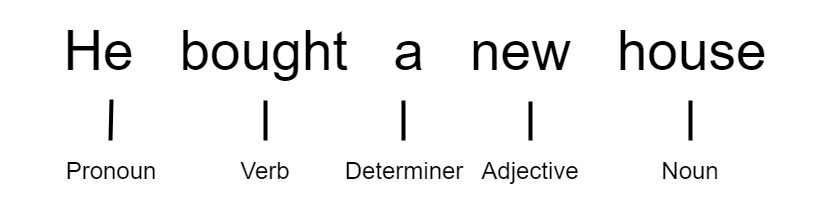
\includegraphics[width=0.6\textwidth]{figures/NLP_example.png}
    \caption{Example of part of speech tagging}
    \label{fig:NLP_example}
\end{figure}

\noindent
This allows a piece of software, such as a chatbot, to take in almost any sentence in a known language and tag the words, making it possible to identify which parts are most important. A problem with part of speech tagging however, is that if given a sentence which is weirdly structured or uses words in an unusual way, it can be hard to tag the words properly. A sentence processed with part of speech tagging might also require further parsing, if it is to be used for advanced sentence processing \cite{NelsonNaturalTechnologies}. 
%\newline\newline
%However when used for having a chatbot give a response to sentences with a predetermined answer, where the sentences can be expected to be relatively simple or if you only want the chatbot to have knowledge about specific subjects and thus know what words to look for. 
